\section{Goal of Research}
\subsection{Impetus}
\frame{
	\frametitle{Role of Thermochemistry}
	\only<1> {\begin{figure}
	\centering
	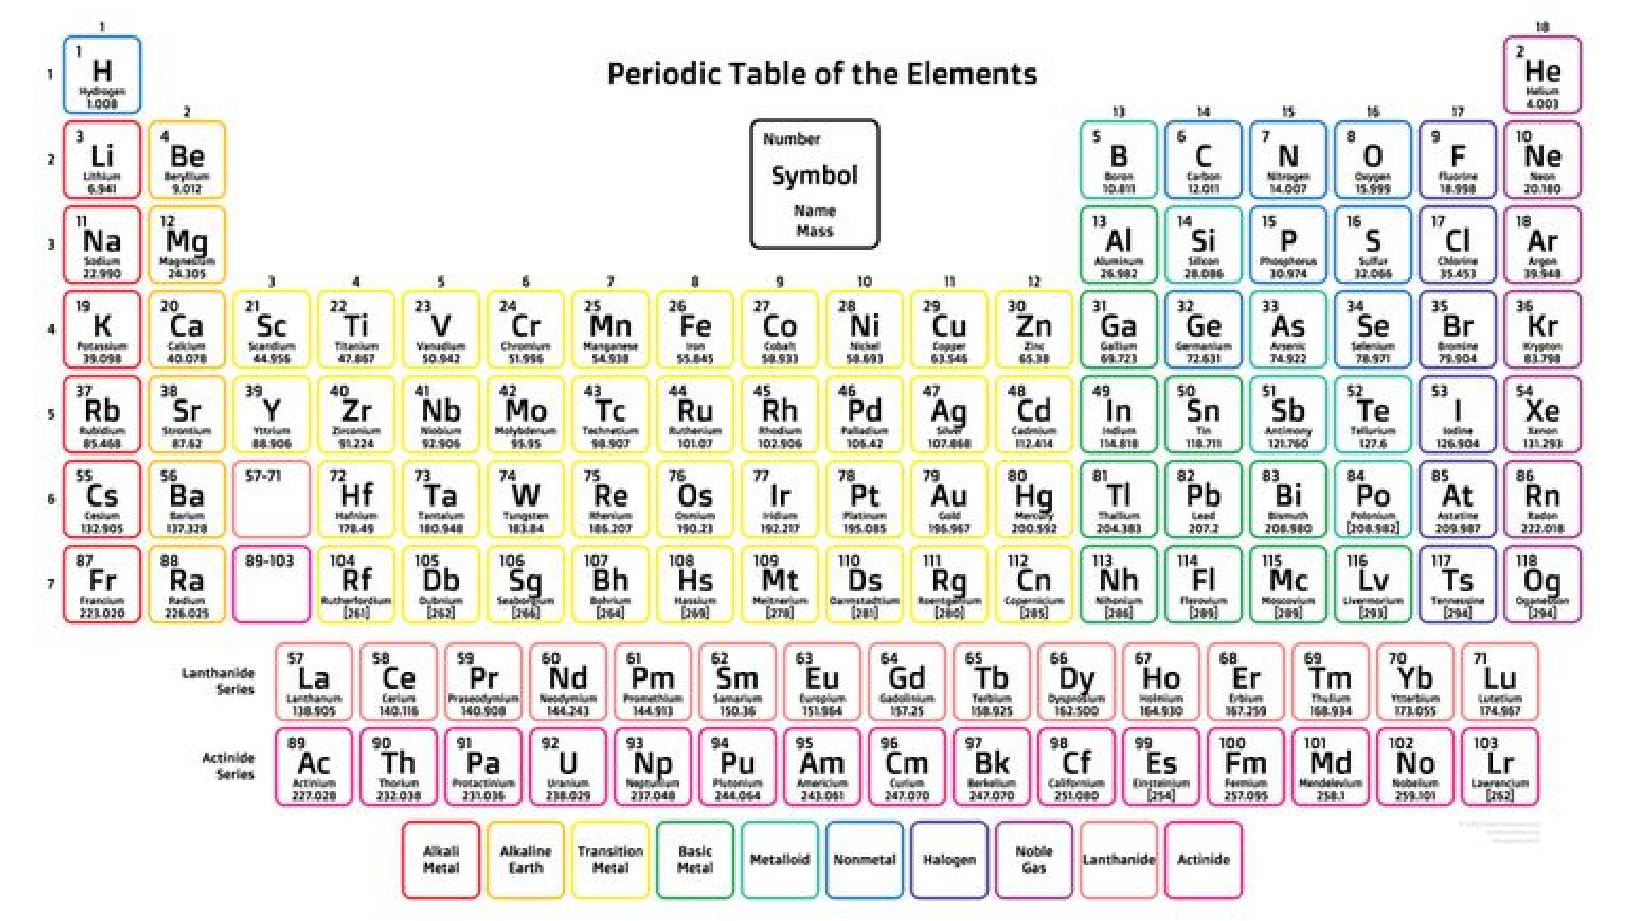
\includegraphics[width=\textwidth]{Figures/PT.pdf}
	\end{figure}
	}
	
	\only<2> {\begin{figure}
	\centering
	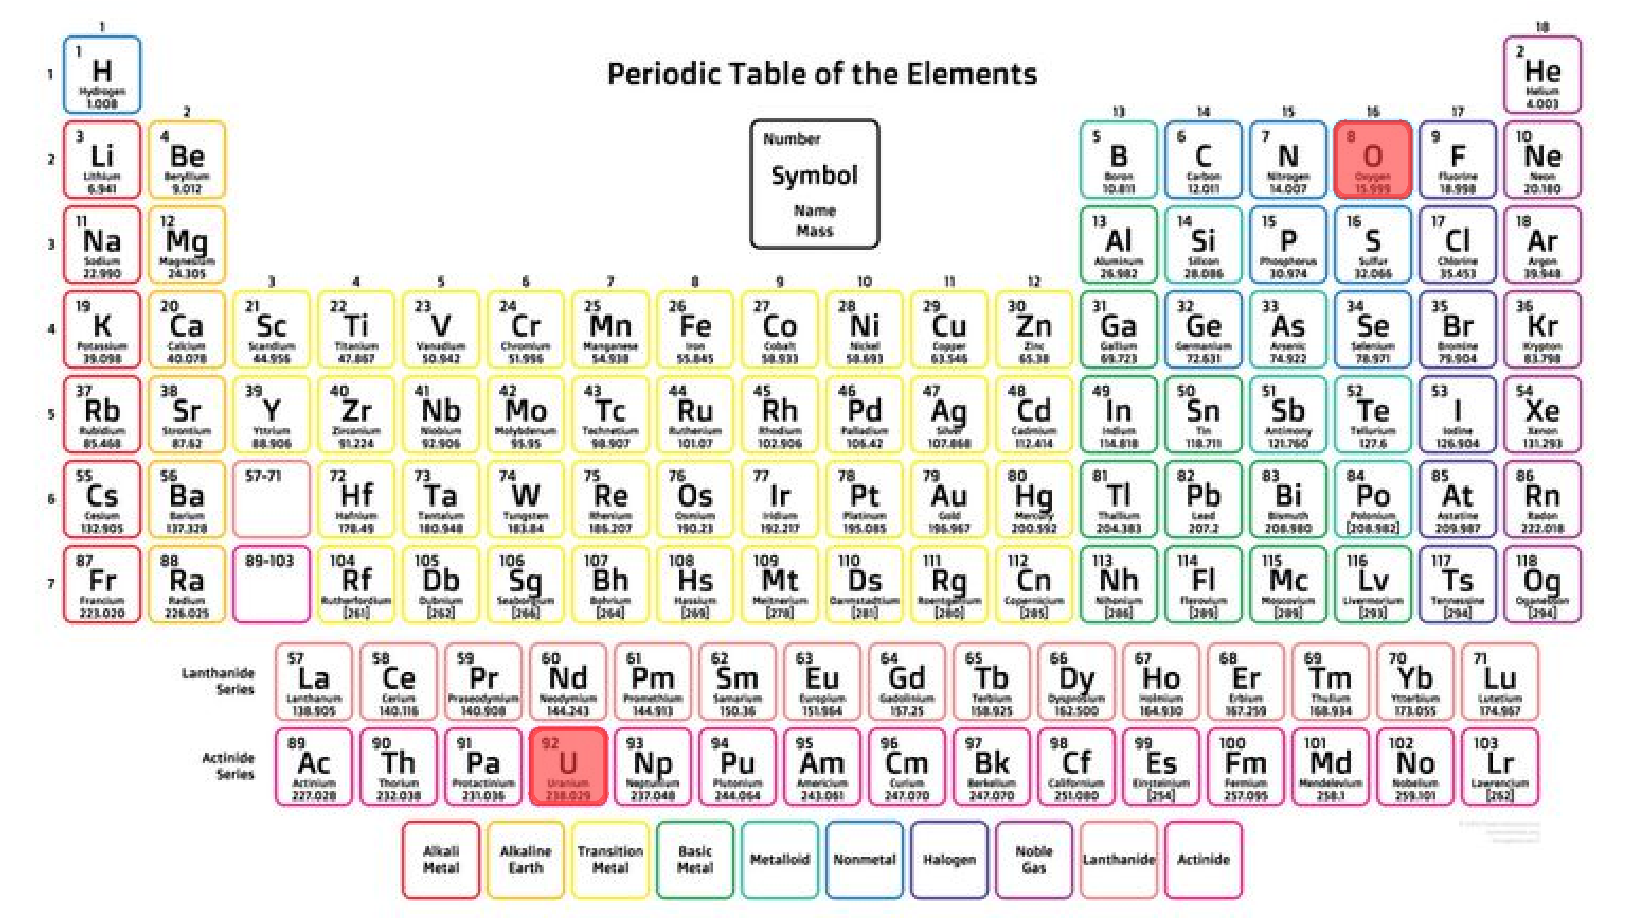
\includegraphics[width=\textwidth]{Figures/PT_BOL.pdf}
	\end{figure}
	}
	
	\only<3> {\begin{figure}
	\centering
	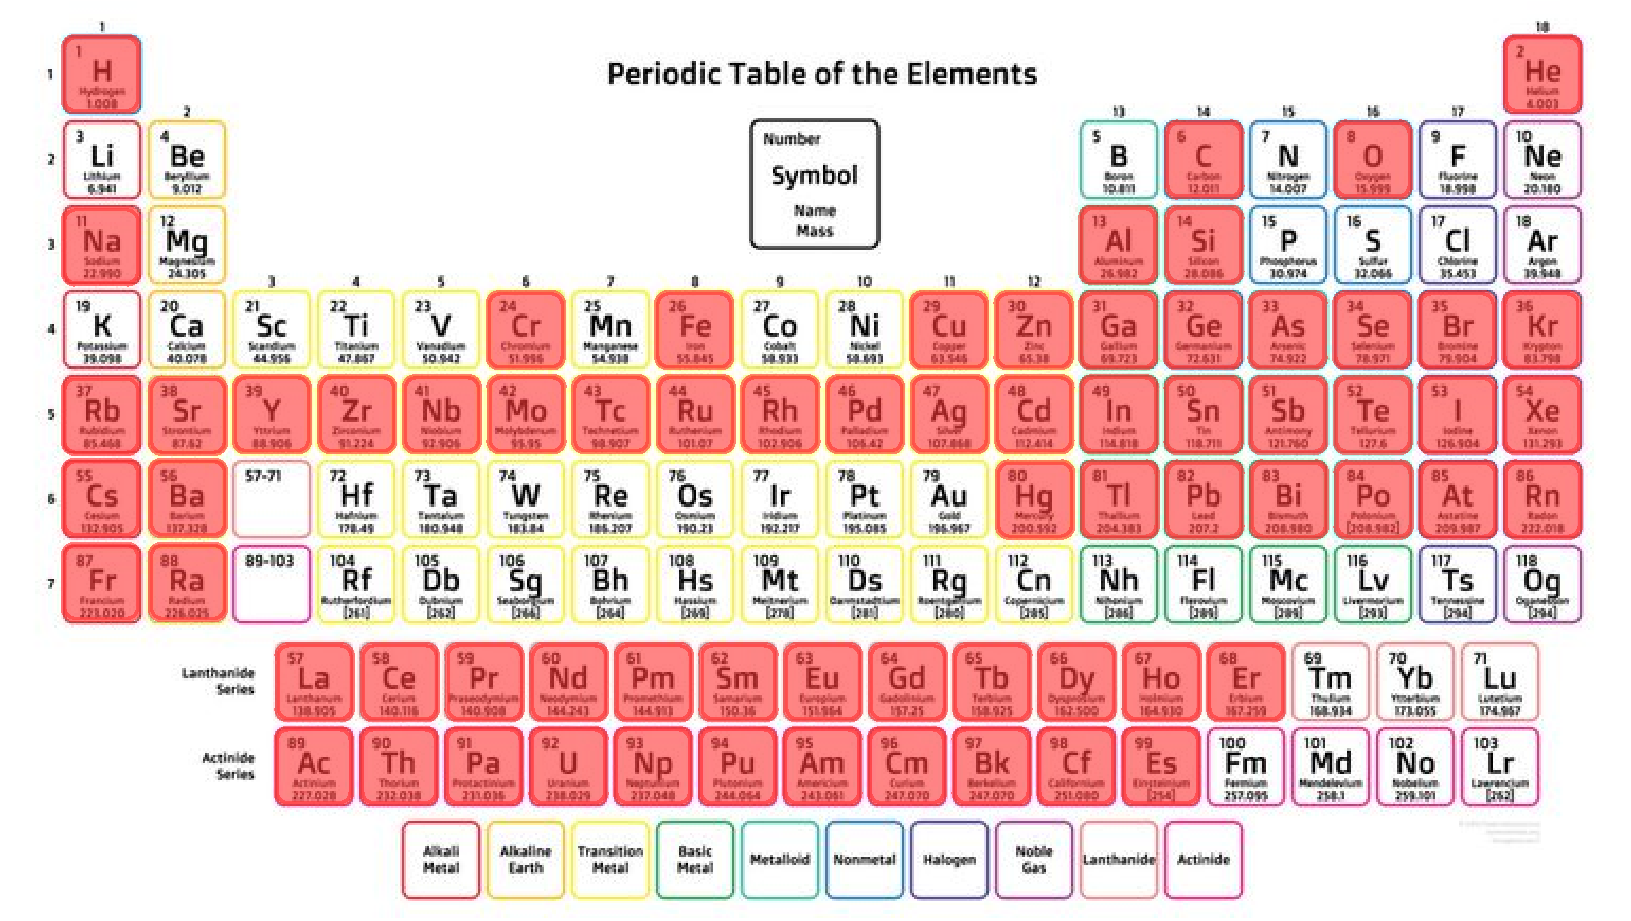
\includegraphics[width=\textwidth]{Figures/PT_EOL.pdf}
	\end{figure}
	}
}

\frame{
	\frametitle{Role of Thermochemistry}
	\onslide<1->{
		\begin{itemize}
			\item<1-> Experiments can not predict the material properties at every single point in the life of a nuclear material.
			\item<1-> Multiphysics simulations have to rely on empirical correlations of material properties, reducing the accuracy of simulations.
			\item<1-> Thermochemistry allows us to capture the effect of compositional evolution on the properties of materials and investigate phenomena which would be impossible to study using only experiments.
		\end{itemize}
	}
	
	\onslide<2->{
	\begin{figure}[htbp]
		\begin{center}
		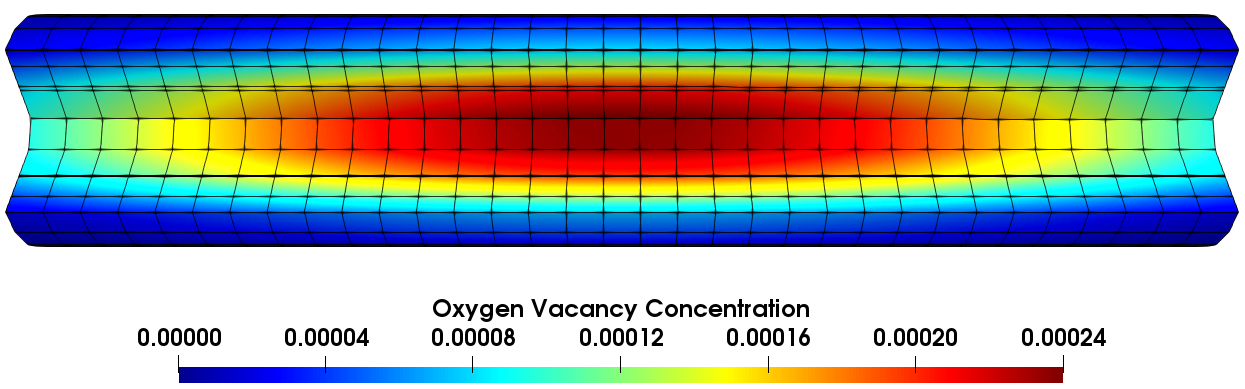
\includegraphics[width=\textwidth]{Figures/O_M}
		\end{center}
	\end{figure}
	\blfootnote{Image - M. Poschmann et al., Technical Report, ORNL. }}
	}

\frame{
	\frametitle{Impetus}
	\begin{itemize}
		\item Direct coupling of thermochemical equilibrium calculations has only recently gained traction in the scientific community.
		\item Equilibrium calculations are extremely costly compared to other finite element based simulations.
		\item The material science community has traditionally relied on using phase diagrams and relatively simple material models in order to save computational cost.
		\item Most thermodynamic equilibrium softwares, such as ThermoCalc and FactSage, are commercial, standalone codes developed in 1970s.
		\item There is little freedom to make improvements or adapt them to specific needs.
		\item Thermochimica is an open-source code developed with the aim of direct coupling with multiphysics codes.
			\begin{itemize}
				\item Written in Fortran 90.
				\item Not developed within the MOOSE framework.
				\item Needs significant work to meet the NQA-1 standards.
			\end{itemize}
	\end{itemize}
}

\subsection{Goal and Outcomes}
\frame{
	\frametitle{Goal and Outcomes}
	\onslide<1->{\begin{block}{Goal of Research} \small
	The goal of this work is to develop a new state-of-the-art thermodynamic equilibrium code for direct integration in mutiphysics framework MOOSE.
	\end{block}}
	\onslide<2->{\begin{block}{Expected Outcomes} \footnotesize
	\begin{enumerate}
		\item Development of a new advanced Gibbs energy minimiser written in C++ within the framework of MOOSE platform.
		\item Full integration within the multiphysics framework MOOSE, with the intent of coupling to the phase field code Marmot. 
		\item Enhanced initialisation algorithms to improve the computational performance.
		\item Investigation and implementation of robust global optimisation schemes to increase reliability and robustness.
		\item Software Quality Assurance  with rigorous verification and testing to comply with the NQA-1 guidelines required to be met for licensing.
	\end{enumerate}
	\end{block}}
}